\documentclass[12pt]{article}

\usepackage[utf8]{inputenc}
\usepackage[T1]{fontenc}
\usepackage[francais]{babel}
%Options: Sonny, Lenny, Glenn, Conny, Rejne, Bjarne, Bjornstrup
% \usepackage[Lenny]{fncychap}
\usepackage{mathpazo}
\usepackage[a4paper, width=150mm, top=25mm, bottom=25mm]{geometry}
\usepackage[colorlinks=true, linkcolor=blue]{hyperref}
\frenchbsetup{StandardLists=true}
\usepackage{enumitem}
\setlist[itemize]{label=\textbullet, topsep=0cm}
\setlist[description]{topsep=0cm}
\usepackage{parskip}
\usepackage{graphicx}
\usepackage{float}
\usepackage{subcaption}

\usepackage{listings}
\lstset{
language=C++,                   
keywordstyle=\color{blue},      
stringstyle=\color{red},        
commentstyle=\color{green},     
basicstyle=\ttfamily,           
numbers=left,                   
numberstyle=\normalsize,        
numbersep=7pt,                  
showstringspaces=false,         
breaklines=true,                
frame=leftline,                 
framerule=2pt,
}

\begin{document}
\pagenumbering{gobble}
\renewcommand{\contentsname}{Sommaire}
\tableofcontents
\newpage

\pagenumbering{arabic}

\section{La programmation avec Python 3}
    \subsection{Introduction}
        Ceci est une petite introduction où on va parler des programmes et des langages de programmations.
        \subsubsection{C'est quoi un programme ??}
            C'est un ensemble d'instructions exécuté par l'ordinateur pour qu'il puisse 
            accomplir une tâche bien précise. On a pour exemple des programmes les navigateurs web 
            (comme chromium, chrome, firefox), qui permettent de visiter les cites et de chatter en ligne ;
            on a aussi les jeux vidéos, les logiciels de retouches de photos \ldots\ etc

            \begin{figure}[H]
                \centering
                \begin{subfigure}[b]{0.49\textwidth}
                    \centering
                    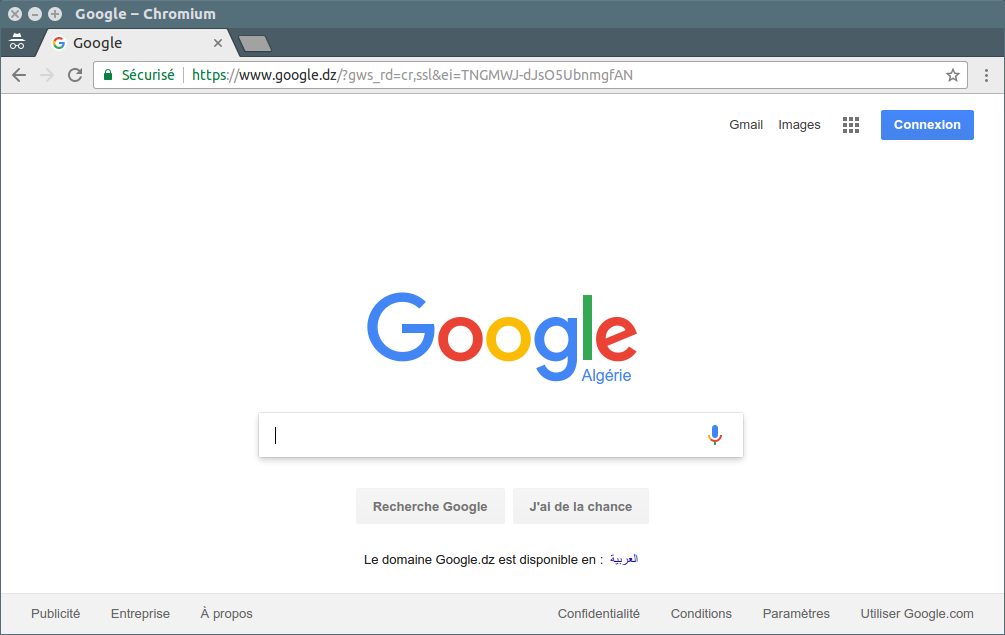
\includegraphics[width=\textwidth, height=2in]{img/1_chrome.png}
                    \caption{Google Chrome}
                \end{subfigure}
                \hfill
                \begin{subfigure}[b]{0.49\textwidth}
                    \centering
                    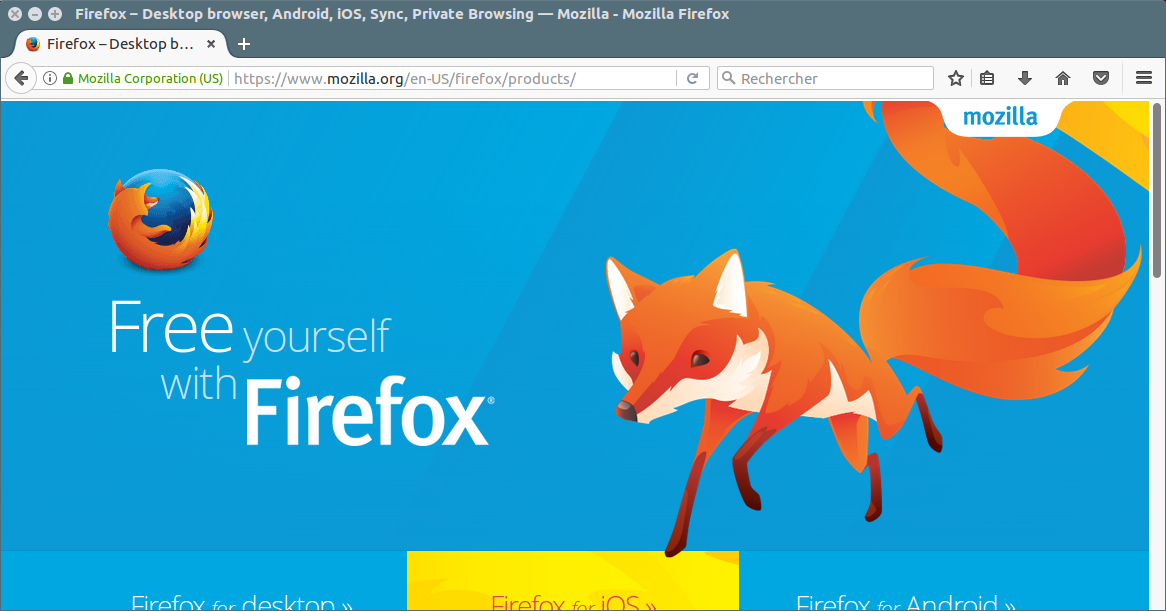
\includegraphics[width=\textwidth, height=2in]{img/2_firefox.png}
                    \caption{Mozilla Firefox}
                \end{subfigure}
            \end{figure}

            \begin{figure}[H]
                \centering
                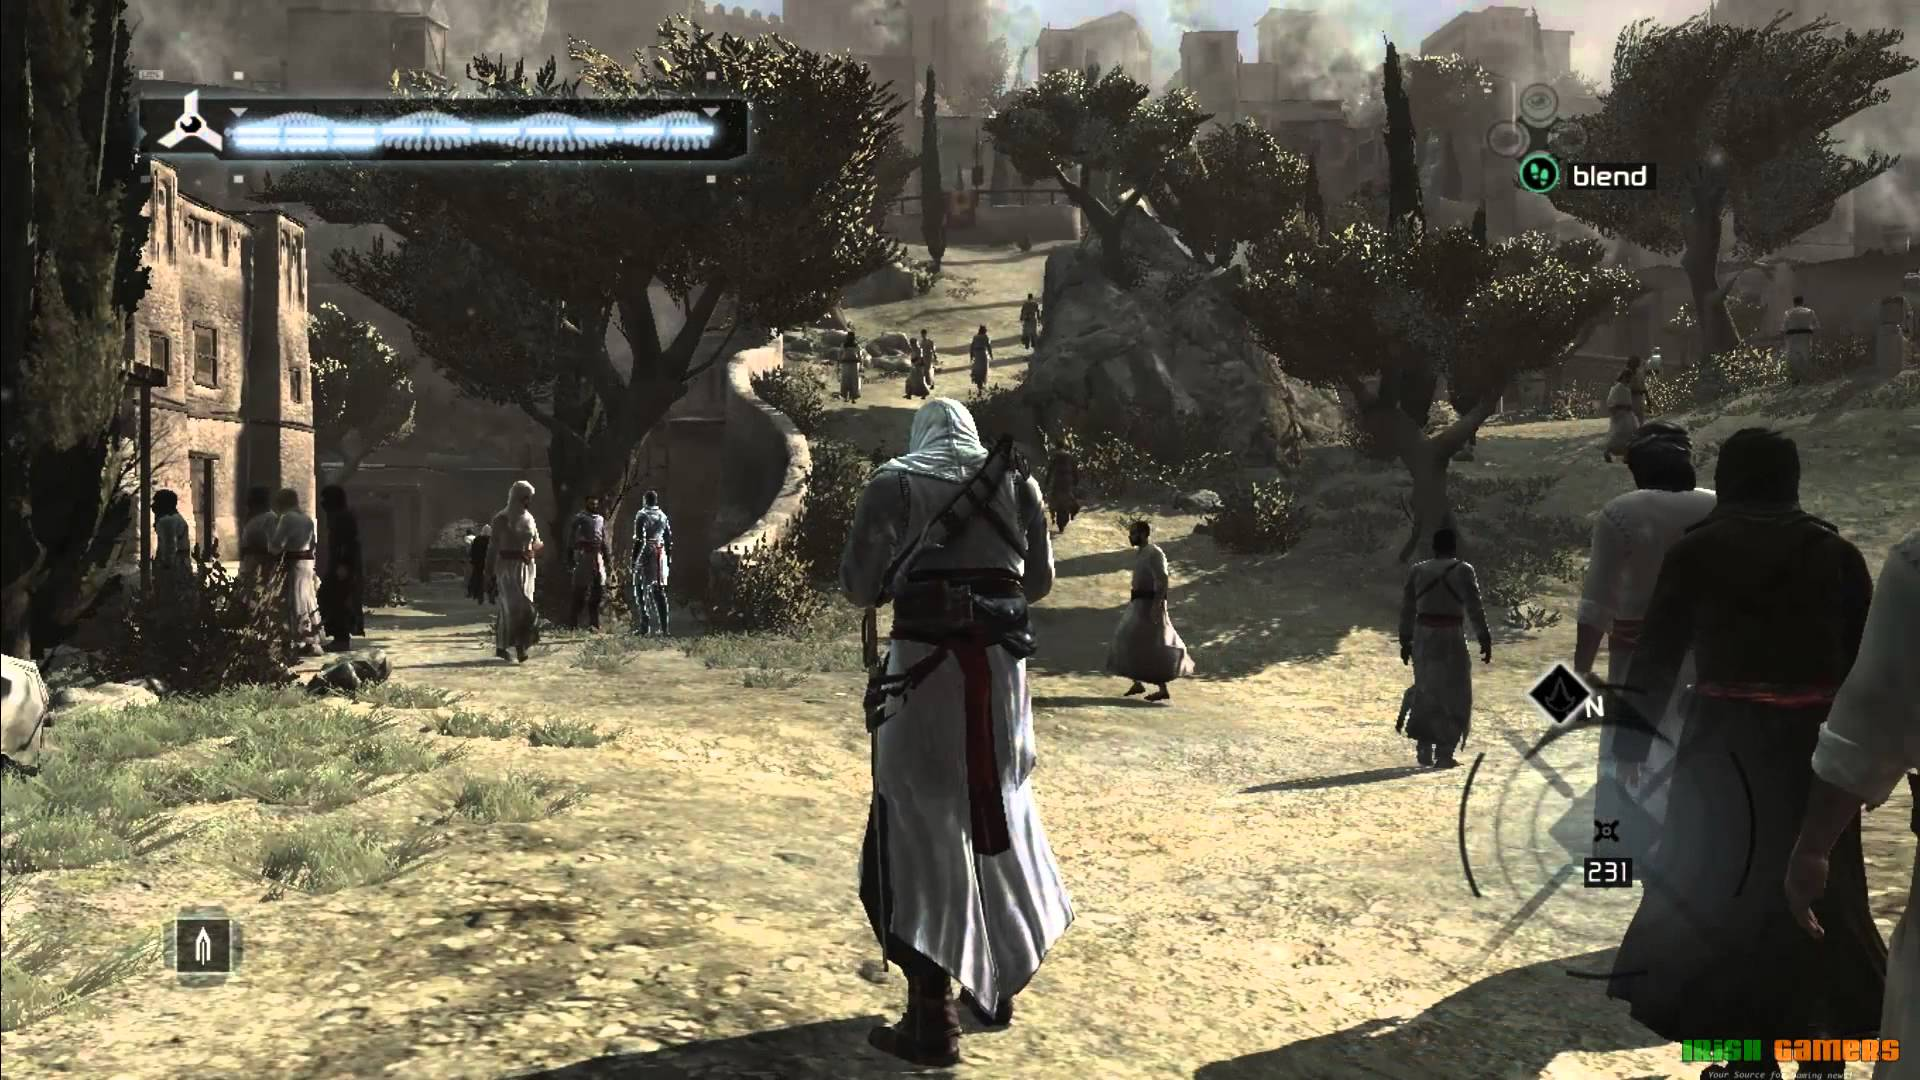
\includegraphics[width=\textwidth]{img/3_assassins_creed.jpg}
                \caption{Le jeu Assassin's Creed}
            \end{figure}
            \begin{figure}[H]
                \centering
                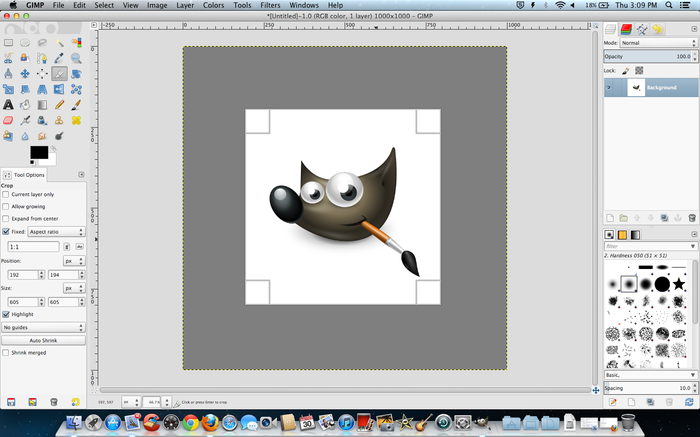
\includegraphics[width=\textwidth]{img/4_gimp.png}
                \caption{Logiciels de retouches ``Gimp''}
            \end{figure}
            % Dans tous les exemples citer avant, on voit que ces programme
            % demande à l'ordinateur d'exécuter des instructions pour qu'il puisse servir; tous ces programmes donnent des instructions bien précise à
            % l'ordinateur pour qu'il puisse accomplir certaines tâches

        \subsubsection{Comment sont crée ces programmes ??}
            L'ordinateur est une machine bête et discipliné qui ne comprend qu'un seul langage, qui est le langage
            \emph{binaire}. Ce langage est une succession de 1 et de 0 comme suit : 
            \begin{lstlisting}[numbers=none]
01101100001100110011000111101011101
            \end{lstlisting}
            
            Donc, normalement, pour créer des programmes, il fallait apprendre ce langage.
            Mais heureusement, les informaticiens ont eu la réflexion de créer d'autres langages intermédiaires 
            (qu'on appel langage de programmation) qui sont beaucoup plus facile que le binaire. Ces langage ont 
            tous le même but : permettre de créer des programmes plus facilement qu'en binaire.
            
            Voici comment cela fonctionne :
            \begin{itemize}
                \item On donne nos instructions à l'ordinateur en utilisant un langage de programmation.
                \item Les instructions sont traduites en binaire grâce à un programme de traduction.
                \item L'ordinateur peut alors lire le binaire et faire ce qu'on l'a demandé.
            \end{itemize}

        \subsubsection{Les langages de programmation les plus connus}
            \begin{description}
                \item[C++ :] La formation est faite par \textsc{Yasser}.
                \item[Java :] La formation est faite par \textsc{Wissam} et \textsc{Sofiane}.
                \item[Python :] C'est la formation à laquelle vous assistez maintenant.
            \end{description}

        \begin{figure}[H]
            \centering
            \begin{subfigure}[b]{0.32\textwidth}
                \centering
                
\includegraphics[width=\textwidth]{img/5_c++.png}
                \caption{Logo C++}
            \end{subfigure}
            \hfill
            \begin{subfigure}[b]{0.32\textwidth}
                \centering
                
\includegraphics[width=\textwidth]{img/6_java.png}
                \caption{Logo Java}
            \end{subfigure}
            \hfill
            \begin{subfigure}[b]{0.32\textwidth}
                \centering
                
\includegraphics[width=\textwidth]{img/7_python.png}
                \caption{Logo Python}
            \end{subfigure}
        \end{figure}
       
        \subsubsection{Compilé vs Interprété}
            Nous avons dit tout à l'heure que les instructions sont traduites en binaire pour que l'ordinateur puisse
            les comprendre et les exécuter. Mais ce qu'on a pas dit c'est qu'il y a deux façons de traduire 
            les instructions : \emph{Compilation} et \emph{Interprétation}.

            \begin{description}
                \item[Compilation :] Avec ce processus, toutes nos instructions sont traduites en binaires à la fois.
                    Ce qui nous donne en résultat un gros fichier binaire qui peut être exécuté directement par
                    l'ordinateur.
                \item[Interprétation :] Avec cette technique, on ne traduit pas tous les instructions en binaires, mais
                    on va plutôt traduire une instruction par instruction à chaque fois qu'on veut exécuter 
                    notre programme. Par exemple, si mon code contient 3 instructions, quand je veux l'exécuter je
                    traduit la première instruction en binaire, et je la passe à l'ordinateur pour qu'il l'exécute ;
                    ensuite je traduit la deuxième instructions, et je la passe à l'ordinateur pour qu'il l'exécute
                    \ldots\ et ainsi de suite jusqu'à la traduction de toute
                    mes instructions.

                    Le programme qui fait l'interprétation est appelé l'\emph{interpréteur}, et dans notre cas on va utiliser
                    l'interpréteur \emph{Python}.
            \end{description}

        \subsubsection{Le langage Python}
            Python est un langage de programmation interprété, facile à apprendre, et très pratique. On cite quelques
            avantages de ce langage :
            \begin{itemize}
                \item Python est facile à apprendre et son code est facile à lire.
                \item Il multiplate-forme, il marche sous Linux, Windows, et Mac OS.
                \item C'est un langage orienté objet (on en parlera de ça dans le prochaines séances).
                \item Il a une bibliothèque tierce qui permet de faire de la programmation web d'une manière très flexible.
                    Cette bibliothèque c'est \emph{Django}.
                \item Il permet de développer très rapidement en utilisant peu de code, et de crée des applications 
                    très complexe avec facilité. Tous ça grâce à son style et à sa bibliothèque standard très complète.
            \end{itemize}

            Pour finir, il faut savoir que les géants de l'informatique comme Google, Yahoo, NASA préférent le langage
            python ; et ce langage est intégré à la quasi totalité des distributions Linux (C'est-à-dire que vous pouvez l'utiliser
            dans ces distributions sans devoir l'installer).

            Juste pour information, il en existe deux versions de python qui ne sont pas compatibles entres eux. Ces
            deux versions sont les 2.x et les 3.x . Nous on va utiliser la version 3.x qui est le future de python.
            % \subsubsection{Les versions de Python}
            %     Python a deux versions qui ne sont pas compatibles entres eux. Ces deux versions sont la version \emph{2.x}
            %     et \emph{3.x}. La version 2.x n'est plus en développement, et il a été pour des raisons de compatibilité
            %     seulement (pour que les anciens programmes écrit en python 2.x continue à fonctionner sans problème).

    \subsection{Les logiciels nécessaires pour la programmation}


    \subsection{Hello World}
    \subsection{Les variables}
        Affichage, lecture des variables.
    \subsection{les opérateurs arithmétique}
    \subsection{Les conditions}
        Explication des structures avec un exemple après chaque petite explication.
    \subsection{Les boucles}
        Explication des structures avec un exemple après chaque petite explication.
    \subsection{Découper le programme en fonctions}
        C'est quoi une fonction. Quelles sont les fonctions que nous avons déjà utilisés. Comment créer nos propres
        fonctions.
    \subsection{TP}
    \subsection{Le help}
        Obtenir le help depuis la console.

\section{La programmation orientée objet}
    \subsection{C'est quoi déjà un objet ?}
    \subsection{Les différents types d'objets disponible}
        On parlera des string, listes, tuples et des dictionnaires.
    \subsection{Les opérations sur les fichiers}
        Ouverture, lecture, écriture des fichiers.
    \subsection{Les chaînes de caractères}
    \subsection{Les listes}
    \subsection{Les tuples}
    \subsection{Les dictionnaires}
    \subsection{TP}

\section{Les bibliothèques standards}
    \subsection{Exécutions des commandes systèmes}
    \subsection{L'aléatoire}
    \subsection{Gestion des mots de passes}
    \subsection{Le réseau}

\section{Allez plus loin}
    Des tutos pour la programmation graphique avec PyQt. Le tuto d'openclassrooms.
\end{document}